\documentclass[a4paper]{article}
\usepackage[utf8]{inputenc}
\usepackage[spanish, es-tabla]{babel}

\usepackage{amsmath}
\usepackage{amsfonts}
\usepackage{amssymb}

\usepackage{float}
\usepackage{graphicx}
\graphicspath{ {./Imagenes/} }

\usepackage{multirow}
\setlength{\doublerulesep}{\arrayrulewidth}

\usepackage{array}
\newcolumntype{C}[1]{>{\centering\let\newline\\\arraybackslash\hspace{0pt}}m{#1}}

\usepackage[american]{circuitikz}

\usepackage{fancyhdr}

\usepackage{units} 

\pagestyle{fancy}
\fancyhf{}
\lhead{22.02 Electrotecnia I}
\rhead{Mechoulam, Mestanza, Lambertucci, Pouthier, Londero}
\rfoot{Página \thepage}


\begin{document}

%%%%%%%%%%%%%%%%%%%%%%%%%%%%%%%%%%%%%%%%%%%%%%%%%%%%%%%%%%%%%%%%%%%%%%%%% 
%								CARATULA								%
%%%%%%%%%%%%%%%%%%%%%%%%%%%%%%%%%%%%%%%%%%%%%%%%%%%%%%%%%%%%%%%%%%%%%%%%% 

\begin{titlepage}
\newcommand{\HRule}{\rule{\linewidth}{0.5mm}}
\center
\mbox{\textsc{\LARGE \bfseries {Instituto Tecnológico de Buenos Aires}}}\\[1.5cm]
\textsc{\Large 22.02 Electrotecnia I}\\[0.5cm]


\HRule \\[0.6cm]
{ \Huge \bfseries Trabajo práctico N$^{\circ}$3}\\[0.4cm] 
\HRule \\[1.5cm]


{\large

\emph{Grupo 5}\\
\vspace{3px}

\begin{tabular}{lr} 	
\textsc{Mechoulam}, Alan  &  58438\\
\textsc{Lambertucci}, Guido Enrique  & 58009 \\
\textsc{Pouthier}, Florian  & 61337 \\
\textsc{Mestanza}, Nicolás  & 57521 \\
\textsc{Londero Bonaparte}, Tomás Guillermo  & 58150 \\
\end{tabular}

\vspace{20px}

\emph{Profesores}\\
\vspace{3px}
\textsc{Muñoz}, Claudio Marcelo\\ 	
\textsc{Ayub}, Gustavo\\ 	

\vspace{100px}

\begin{tabular}{ll}

Presentado: & 17/05/19\\

\end{tabular}

}

\vfill

\end{titlepage}


%%%%%%%%%%%%%%%%%%%%%%%%%%%%%%%%%%%%%%%%%%%%%%%%%%%%%%%%%%%%%%%%%%%%%%%%% 
%								INFORME									%
%%%%%%%%%%%%%%%%%%%%%%%%%%%%%%%%%%%%%%%%%%%%%%%%%%%%%%%%%%%%%%%%%%%%%%%%%

\section*{Introducción}

El desarrollo de la experiencia consiste en el análisis de un circuito en triangulo, alimentado por corriente trifásica. Se utilizó cargas no balanceadas alternando entre valores resistivos, inductivos y resistivos e inductivos en paralelo.

\section*{Desarrollo de la experiencia}

Se conectaron las cargas y los instrumentos de la forma que se muestra en la imagen (\ref{fig:circuito}).

\begin{figure}[H]
	\centering
	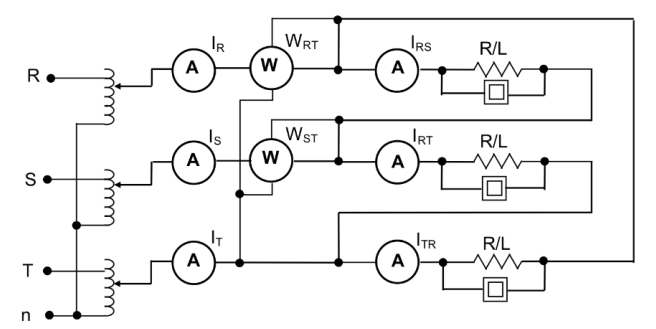
\includegraphics[width=0.8\textwidth]{Circuito}
\caption{Circuito trifásico analizado, alternando las cargas.}
	\label{fig:circuito}
\end{figure}

De esta forma, se obtuvieron los siguientes valores:

\begin{table}[H]
\centering
\begin{tabular}{|c|c|c|c|c|c|c|c|c|c|c|c|}
\hline
\multicolumn{3}{|c|}{\textbf{Fase}} & \textbf{$U_{RS}$} & \textbf{$U_{ST}$} & \textbf{$U_{TR}$} & \textbf{$I_{RS}$} & \textbf{$I_{ST}$} & \textbf{$I_{TR}$} & \textbf{$I_{R}$} & \textbf{$I_{S}$} & \textbf{$I_{T}$} \\ \hline
\textbf{RS} & \textbf{ST} & \textbf{TR} & \textbf{V} & \textbf{V} & \textbf{V} & \textbf{A} & \textbf{A} & \textbf{A} & \textbf{A} & \textbf{A} & \textbf{A} \\ \hline
\textbf{R} & \textbf{R} & \textbf{R} & 140 & 137,2 & 137,5 & 2,075 & 2,04 & 1,83 & 2,075 & 2,05 & 3,7 \\ \hline
\textbf{L} & \textbf{L} & \textbf{L} & 140 & 137,2 & 137,5 & 1,31 & 2,21 & 1,42 & 1,55 & 2,2 & 2,9 \\ \hline
\textbf{R/L} & \textbf{R/L} & \textbf{R/L} & 140 & 137,2 & 137,5 & 1,97 & 3,22 & 2,22 & 3 & 3,4 & 4,5 \\ \hline
\textbf{R} & \textbf{R/L} & \textbf{L} & 140 & 137,2 & 137,5 & 1,29 & 2,94 & 2,06 & 1,05 & 2,95 & 4,15 \\ \hline
\end{tabular}
\label{tabla:1}
\caption{Mediciones de corrientes del circuito.}
\end{table}

\begin{table}[H]
\centering
\begin{tabular}{|c|c|c|c|c|c|c|}
\hline
\multicolumn{3}{|c|}{\textbf{Fase}} & \textbf{$W_{RT}$} & \textbf{$W_{ST}$} & \textbf{P} & \textbf{Q} \\ \hline
\textbf{RS} & \textbf{ST} & \textbf{TR} & \textbf{W} & \textbf{W} & \textbf{W} & \textbf{VAR} \\ \hline
\textbf{R} & \textbf{R} & \textbf{R} & 242 & 236 & 478 & 10,39 \\ \hline
\textbf{L} & \textbf{L} & \textbf{L} & 196 & 100 & 296 & 166,28 \\ \hline
\textbf{R/L} & \textbf{R/L} & \textbf{R/L} & 396 & 132 & 528 & 457,26 \\ \hline
\textbf{R} & \textbf{R/L} & \textbf{L} & 116 & 248 & 364 & -228,63 \\ \hline
\end{tabular}
\label{tabla:2}
\caption{Mediciones de potencia del circuito.}
\end{table}

De esta forma, se grafica fasorialmente las tensiones de fase y las corrientes de linea de cada circuito.

\begin{figure}[H]
	\centering
	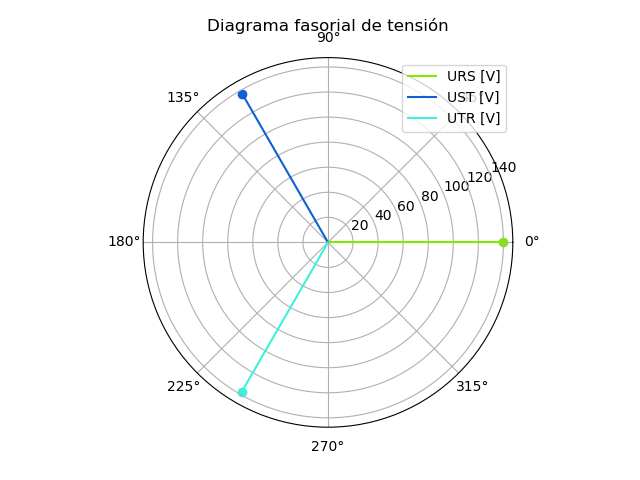
\includegraphics[width=0.8\textwidth]{Tensiones}
\caption{Diagrama fasorial de tensiones. Constante para cada circuito.}
	\label{fig:tensiones}
\end{figure}

\begin{figure}[H]
	\centering
	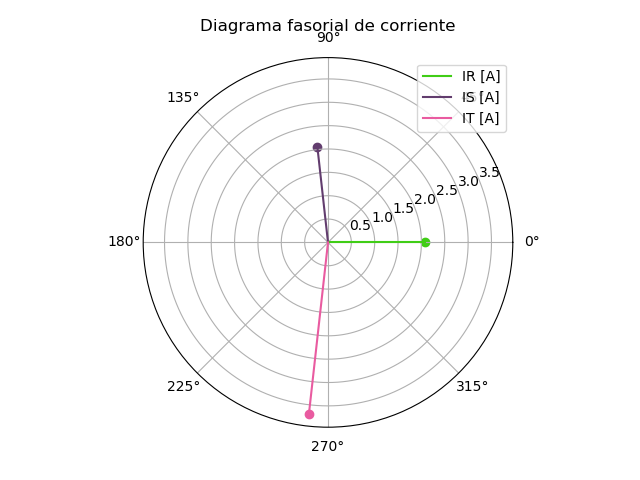
\includegraphics[width=0.8\textwidth]{Corriente-RRR}
\caption{Diagrama fasorial de corriente para el circuito de tres resistencias.}
	\label{fig:corriente-rrr}
\end{figure}

\begin{figure}[H]
	\centering
	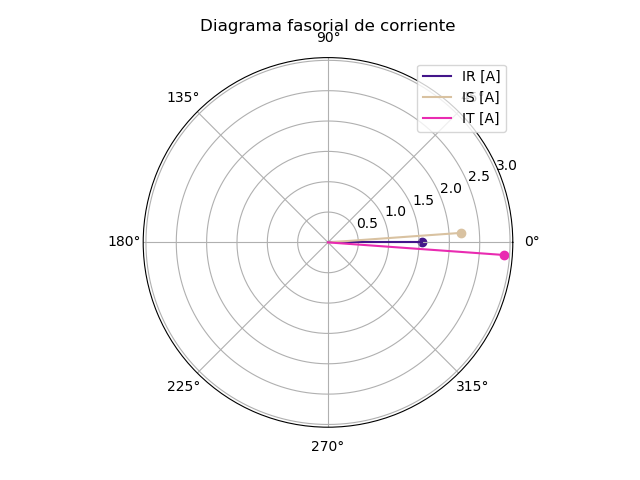
\includegraphics[width=0.8\textwidth]{Corriente-LLL}
\caption{Diagrama fasorial de corriente para el circuito de tres inductancias.}
	\label{fig:corriente-lll}
\end{figure}

\begin{figure}[H]
	\centering
	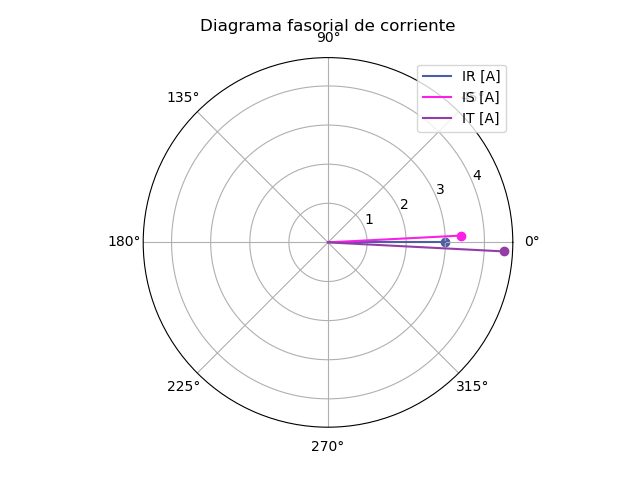
\includegraphics[width=0.8\textwidth]{Corriente-PARALELO}
\caption{Diagrama fasorial de corriente para el circuito de resistencias e inductancias en paralelo.}
	\label{fig:corriente-par}
\end{figure}

\begin{figure}[H]
	\centering
	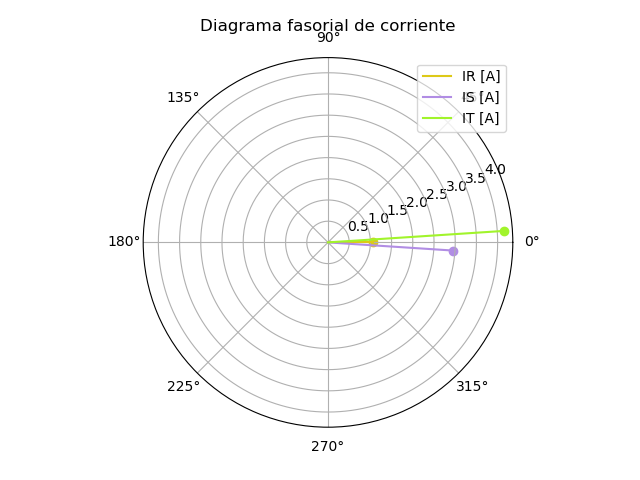
\includegraphics[width=0.8\textwidth]{Corriente-RPARALELOL}
\caption{Diagrama fasorial de corriente para el circuito de una resistencias, inductancias y resistencia e inductancia en paralelo.}
	\label{fig:corriente-rlpar}
\end{figure}


\section*{Conclusión}

Luego de realizar el experimento utilizando el circuito en triángulo alimentado por una corriente 
trifásica con cargas no balanceadas, pudimos observar los efectos esperados para las distintas situaciones presentadas en cuanto a las cargas para cada fase.


Con respecto al cálculo de la potencial total, se utilizó el método de Aaron con dos vatímetros para poder obtener la misma, donde calculó la potencia total como la potencia suministrada para cada una de las fases. La potencia se midió con dos vatímetros monofásicos conectados según se mostró en la Figura 1 y la suma de 
ambas resulta la potencia activa del circuito. Más allá de ello, se puede observar con los datos obtenidos
como varía la potencia total en cada caso, haciendo que la potencia aparente al agregar elementos inductivos en las cargas de las fases aumente y para el primer caso (tres resistencias en las cargas) sea casi nula.


El gráfico de las tensiones muestra la tensión de cada fase aplicada, teniendo una diferencia de fase entre cada una de ellas de 120 grados y es constante para las cuatro situaciones analizadas.


Para el caso de las tres resistencias, observamos un desfasaje que se genera en las corrientes no tan abrupto como en el resto de los casos debiéndose esto a las cargas utilizadas (Resistencias cuyo desfasaje generado es 0). Luego, en los siguientes casos vemos una variación en la fase aun más notable para las corrientes de cada fase, y obviamente se observa efectos en cuanto el módulo de dicha corriente que se condicen con las cargas presentadas para cada caso.

\end{document}
